\documentclass{article}
\usepackage[utf8]{inputenc}
\usepackage{natbib}
\usepackage{graphicx}
\usepackage{textcomp}
\usepackage{amsmath}
\usepackage[T1]{fontenc}
\usepackage{graphicx}
%\graphicspath{ {images/} }
\usepackage{amssymb}
\usepackage{url}
\usepackage{float}

\title{Assignment 3}
\author{Pratik Gaikwad}

\begin{document}

\maketitle

\section{Hash functions and applications}
    \paragraph{Question 1:} What is a \emph{collision-resistant}(CR) \emph{hash function} H? When is a CR hash function \emph{h} also a \emph{compression} function? what is \emph{random oracle} $\mathcal{H}$?
    
    \paragraph{Answer: \newline}
        A hash function $\prod = (Gen, H)$ is collision resistant if for all \emph{probabilistic polynomial time} adversaries $\mathcal{A}$ there exists a \emph{negligible} function negl such that:
        \begin{center}
            \begin{math}
                Pr[Hash-coll_{\mathcal{A},\prod}(n)=1] \leq negl(n)
            \end{math}            
        \end{center}
        
        In other words, it should be very hard for the function to generate same hash values for two different messages.
        
        If the above CR function \emph{h} maps $\mathit{l}^{\prime}(n)$-bit string to a $\mathit{l}(n)$-bit string with $\mathit{l}^{\prime}(n) > \mathit{l}(n)$, then CR is called \emph{compression} function.
        
        Let suppose $\mathcal{H}(m)$ be the uniform output domain of the oracle $\mathcal{H}$. Then $\mathcal{H}$ will be called \emph{random oracle} if for every unique query made using different \emph{m}, a truly random value of hash from \emph{uniform} output domain $\mathcal{H}(m)$ is returned.
        
    \paragraph{Question 2:} Suppose that a hash function $\mathcal{H}$ is devised as the Merkle-Damgard transform over \emph{compression} function \emph{h}. What is this transform and what is its practical importance? If \emph{h} is CR, is $\mathcal{H}$ also CR and why? if \emph{h} is random oracle, is $\mathcal{H}$ also a random oracle and why?
    
    \paragraph{Answer: \newline}
        The transform of $\mathcal{H}$ over \emph{h} is building collision resistant \emph{hash} function from collision resistant \emph{compression} function. Using Merkle-Damgard transform we can build, in practice, collision resistant hash function by creating collision resistant compression function with small message blocks.\newline
        
        If \emph{h} is CR then $\mathcal{H}$ is also a CR. We can prove this by proof of contradiction using induction from the end of message travelling towards beginning of the message based on working on Merkle-Damgard transformation. \newline
        We assume that there exists a collision on $\mathcal{H}$ i.e. two distinct messages with equal length hashed to same hash value. 
        In Merkle-Damgard output of the transform is one of the input to next transform, that means second to last message blocks are hashing to same value or the padding block is equal. Conclusion from this arguments is, in order to get collision for \emph{h} we are stating that arguments to compression function are distinct. but again if we assume that this arguments are same, then we are using induction to travel towards the beginning of message. so for two non-equal messages with same length, there must be a collision for \emph{h} based on our above assumption or both the message are identical with their blocks. This contradicts our basic assumption that we didn't have collision over $\mathcal{H}$. And hence if \emph{h} is CR, it proves by induction that $\mathcal{H}$ is also a CR \cite{mdpbyprofDanBoneh}.\newline
        
        Even if \emph{h} is random oracle $\mathcal{H}$ will not be a random oracle since $\mathcal{H}$ is a deterministic function. i.e. for every \emph{same} input \emph{x}, $\mathcal{H}$ will produce same output $\mathcal{H(x)}$. And hence $\mathcal{H}$ is not random.
        
        
    \paragraph{Question 3:} Let $h:{\{0,1\}}^{2n} \rightarrow {\{0,1\}}^n$ be a compression function and consider the function $f:{\{0,1\}}^n \times{{\{0,1\}}^n} \rightarrow {\{0,1\}}^n$ that is a keyed function defined as $f_k{(x)} = h(k||x)$. Show that if \emph{h} is modeled as a \emph{random oracle} and \emph{k} is chosen \emph{uniformly at random} k $\leftarrow {\{0,1\}}^n$, then $f_k{(x)}$ is:
        \begin{enumerate}
            \item a pseudo-random function (PRF);
            \item a secure message authentication code (MAC); and
            \item a secure (i.e., binding and hiding) commitment.
        \end{enumerate}
        
        \paragraph{Answer: \newline}
        \begin{enumerate}
            \item a pseudo-random function (PRF): \newline
                For two different inputs, the calculation will be 
                $f_k(x_1)= h(k||{x_1})$\newline
                $f_k(x_2)= h(k||{x_2})$ \newline
                here $k={\{0,1\}^n}$ \newline
                The adversary basically guesses the output. In ppt, this is negligible. This indicates that PRF doesn't reveal anyting about input values. and thus below definition of the security is captured.
                \begin{center}
                    \begin{math}
                        |Pr[D^{F_k(.)}(1^n)=1]-Pr[D^{f(.)}(1^n)=1]| \leq negl(n)
                    \end{math}
                \end{center}
            
            \item A secure message authentication code(MAC): \newline
                The tag for the mac will be calculated as $f_k(x) = h(k||x)$. For another message $x^{\prime}$, where x and $x^{\prime}$ are randomly chosen, the tag $t^{\prime}$ is calculated as 
                \begin{center}
                    \begin{math}
                        t^\prime = h(t||x^\prime) \newline
                        t^\prime = h(h(k||x)||x^\prime) \newline
                        t^\prime = \mathcal{H}(k||x||x^{\prime}) = Mac_k(x||x^{\prime})
                    \end{math}
                \end{center}
                
                Since two message m and $m^{\prime}$ are different with $h(k||m) = h(k||m^{\prime})$ we can conclude that h(x) = h(y)\newline
                s.t. $x = k||m, y = k||m^{\prime} $
                Since \emph{f} is \emph{PRF}, this MAC is also secure. This can be concluded from the definition of the MAC as follows:
                \begin{center}
                    \begin{math}
                        HMac_k[m] = H^s[(k\oplus{opad})||H^s[(k\oplus{ipad})||m]]
                    \end{math}
                \end{center}
            
            \item A secure (i.e., binding and hiding) commitment: \newline
                \begin{enumerate}
                    \item binding: $\mathcal{A}$ selects two messages $m_1 \neq m_2$ as \emph{h} is a CR it indicates $f_k(x_1) \neq f_k(x_2)$. Which means that $\mathcal{A}$ can do no better than guessing and can not win.
                    \item hiding: $\mathcal{A}$ selects two messages such that $f_k(x_1) = h(k||x_1) and f_k(x_2) = h(k||x_2)$. Using a random bit b cipher text $c_b$ is given to $\mathcal{A}$. Because \emph{h} is random oracle, $\mathcal{A}$ can not guess with probability better than $\frac{1}{2}$. Thus commitment hides the message.
                \end{enumerate}
            
        \end{enumerate}
    
\section{Computational number-theoretic assumptions}
    If $\mathcal{G}$ is a \emph{cyclic} group of \emph{prime} order \emph{p} and \emph{g} a \emph{generator} of $\mathcal{G}$, then the discrete-log problem is defined as: Given (a description of G), \emph{p, g} and an element $h \in \mathcal{G}$, find the discrete log of \emph{h}.
    
    \paragraph{Question 1:} What is the \emph{discrete log} of \emph{h} and what constitutes a \emph{brute-force} solution for this problem?
    \paragraph{Answer: \newline}
        Since $h \in \mathcal{G}$ and \emph{g} is given as generator of $\mathcal{G}$ which is also a \emph{cyclic} group. Then we can write $h = g^x$ for some x. \newline
        The discrete log of \emph{h} to the base \emph{g} is defined as \emph{x}. i.e. finding the correct power when \emph{g}, \emph{h} and order \emph{p} of $\mathcal{G}$ are given.\newline
        
        A \emph{brute-force} solution to this problem would be raising the generator to all the powers(x) from 1, 2, ... , p-1 to get the exact \emph{h}. 
        
    \paragraph{Question 2:} The \emph{DL assumption} postulates that certain instances of this problem are \emph{computationally hard} for PPT adversaries. (A) Provide two different descriptions of such instances (related to the choice of \emph{h}) and explain why there are equivalent. (B) How should the security parameter $1^n$ relate to \emph{p} for the DL assumption to be reasonable (i.e., not trivially refutable)?
    \paragraph{Answer: \newline}
        \begin{enumerate}
            \item The messages are created by raising generator to various powers and performing modulus operation. This results in two same values for separate powers. So when prime number used in large, then the calculation of discrete of log is very hard. Because from Fermat's theorem we can conclude that there are no three numbers greater than which satisfies below equation $a^n + b^n = c^n$.
            \item 
        \end{enumerate}
        
    \paragraph{Question 3:} What are the \emph{computational} Diffie-Hellman (CDH) and \emph{decisional} Diffie-Hellman (DDH) assumptions? How do they relate to each other and the DL assumption? (Does the DDH assumption imply the CDH assumption and why? Does the CDH assumption imply the DL assumption and why? Amongst all three assumptions, which is the strongest and which the weakest?) Why is the security of the Diffie-Hellman key-agreement protocol based on the DDH assumption?
    \paragraph{Answer: \newline}
        Both CDH and DDH are the assumptions within \emph{cyclic} group about solving a computational problem. \newline
        
        \underline{Computational Diffie-hellman assumption}: This assumption states that a computational problem within a cyclic group is \emph{hard}. Hence for the given group $\mathcal{G}$ with order \emph{p} and any generator \emph{g} and random $a, b \in \{0, ... , p-1\}$, it is computationally improbable in probabilistic polynomial time to compute $g^{ab}$ when $g,\ g^a,\ g^b$ are given. \newline
        The CDH assumption is related to DL in the sense that it is hard to compute \emph{discrete log} of a value with base \emph{g} in $\mathcal{G}$. If calculation of DL was trivial in PPT, then to compute $g^{ab}$ in CDH all one has to do is:\newline
        \begin{enumerate}
            \item compute \emph{a} by taking discrete log of $g^a$ with base \emph{g}
            \item compute $g^{ab}$ by raising $g^b$ to the power \emph{a} i.e. ${g^b}^a$.
        \end{enumerate}
        
        \underline{Decisinal Diffie-hellman assumption}: This assumption states that a computational hard problem within a cyclic group. Hence for the given group $\mathcal{G}$ with order \emph{p} and any generator \emph{g} and random $a, b \in \{0, ... , p-1\}$, if we are given the values of $g^a,\ g^b,\ g^c$ we need to conclude if $g^c = g^{ab}$ without actually calculating \emph{a, b or c}.\newline
        The DDH assumption is related to DL in the sense that it is computationally hard to compare $g^{ab},\ g^a,\ g^b$. If calculation of DL was trivial in PPT, then to compare $g^{ab}$ in DDH all one has to do is:\newline
        \begin{enumerate}
            \item compute \emph{a} by taking discrete log of $g^a$ with base \emph{g}
            \item compute \emph{b} by taking discrete log of $g^b$ with base \emph{g}
            \item compute \emph{ab} by taking discrete log of $g^{ab}$ with base \emph{g}
            \item compare if $a \times{b} = ab$
        \end{enumerate}
        
        They both are related to each other such that in both the cases, discrete log needs to be calculated at any steps.\newline
        
        Yes DDH assumption implies CDH, since in CDH we need to compute $g^{ab}$ whereas in DDH, we need to compare it from the given values i.e. make 3 computations. Yes CDH assumption imply DL since to compute $g^{ab}$ we need to first compute DL of $g^a$ in PPT before computing $g^{ab}$. Hence if DL is easy to calculate the CDH is also easy to calculate.\newline
        For some groups DDH is stronger while in others CDH but DDH is considered as stronger for large \emph{p}. Both of them are as strong as DL. \newline
        
        In Deffie-Hellman key agreement both parties select two random relative prime numbers each and raise them to a power of same generator and share the computed number to each other so that other parties can raise the received number to the number they have chosen. I.e. Let's say Alice select \emph{a} and Bob select \emph{b} with generator \emph{g}. Alice computes $g^a$ and Bob computes $g^b$ and they share computed values with each other. Upon receiving these values, Alice then computes ${g^b}^a$ whereas Bob computes ${g^a}^b$ and thus both ends up having same value i.e. $g^{ab}$. In DDH, we need to compute $g^{ab}$ from both $g^{a}$ and $g^{b}$. Since DL computation computation is not easy, its tough to calculate $g^{ab}$ and compare. Hence DDH assumption is used in DH key-agreement.
        
    \paragraph{Question 4:} How do the following three assumptions \emph{qualitatively} compare with each other?
    \begin{enumerate}
        \item The has function SHA-256 realized a random oracle h(.)
        \item The block cipher AES with key \emph{k} realizes a PRF $F_k(.)$.
        \item The discrete log problem is computationally hard in cyclic groups of prime order.
    \end{enumerate}
    \paragraph{Answer: \newline}
        \begin{enumerate}
            \item SHA256 is one way fixed length CR hash function with random oracle \emph{h(.)}. It is one of the compression function which reduces large input in fixed length small output. Since it is one way, it is nearly impossible to relate input with output.
            \item AES is a symmetric encryption which uses a pseudorandom function $f_k$ for 128 bits. Since it is symmetric key encryption, both participants in the communication must know secret key for encryption and decryption. Plaintext message can be obtained from encrypted message if secret key is know.
            \item Discrete log: It is a hard mathematical problem to calculate of the power in the exponent from the value. In a cyclic group $ \emph{G} $ with order p prime, let's assume \emph{g} is the generator. Then $ \forall \ h \in \emph{G} $  , $ \exists x $ s.t. $ g^x= h $ . So, it takes as input the generator g and raise it to power to get the elements (outputs). Thus, we have to compute $ g^{x_i}$  ,$ \forall \ i $
        \end{enumerate}
        
\section{Public-key encryption and signatures}
    \paragraph{Question 1:} Compared to secret-key cryptography, how does the use of \emph{public-key} cryptographic schemes (say for the secrecy and integrity of communications) change the \emph{key-management} problem?
    \paragraph{Answer: \newline}
        In secret-key or \emph{symmetric}-key cryptography same key is used for both encryption and decryption. Hence the key must kept hidden or secret for both secrecy and integrity of the communication. \newline
        Where as in public-key cryptography \emph{two} different keys are used for encryption and decryption. In usual case, the \emph{public}-key is used for encryption by the message sender while corresponding \emph{private}-key is used for decryption of the message by the recipient. So the \emph{public}-key can be made available to anyone who wishes to encrypt message. However the message can not be decrypted without corresponding \emph{private}-key. And hence only \emph{private}-key must be very well managed.\newline
        Public-key and private-key form a pair using various algorithms. Hence it is very hard to create two pair of \emph{same} public and private keys. so key management and distribution is a easier than \emph{private}-key encryption scheme.
        
    \paragraph{Question 2:} Recall the basic game-based definition for computational secrecy, EAV-security depicted in Figure 1, that is required for public-key encryption. Show why \emph{no perfectly secure public-key encryption scheme exists}, i.e., EAV-security cannot be satisfied \emph{unconditionally}.
    \paragraph{Answer: \newline}
    
    %Secure PK Encryption impossible when P=NP, as deriving K-1 from K is in NP.

\section{Merkle tree}
    Recall the secure data outsourcing model described in Figures 2, 3 and 4. To answer the questions below, use any programming language of your choice that supports the SHA-256 hash function h.
    
    \paragraph{Question 1:} By applying the hash function h on messages of variable lengths, experimentally evaluate the time $T_h(x)$ that is required to hash a message \emph{m} as a function of its length $x = |m|$ in bytes. Plot a graph for function $T_h(x)$. What do you observe about $T_h(x)$? How does this confirm the design method used in the design of the SHA-2 family of hash functions?
    \paragraph{Answer:\newline}
        The plot of time required to calculate SHA256 hash value of variable length message is as below. Here variable length message was obtained using the contents of the files of lecutre notes.
        
        \begin{figure}[H]
            \centering
            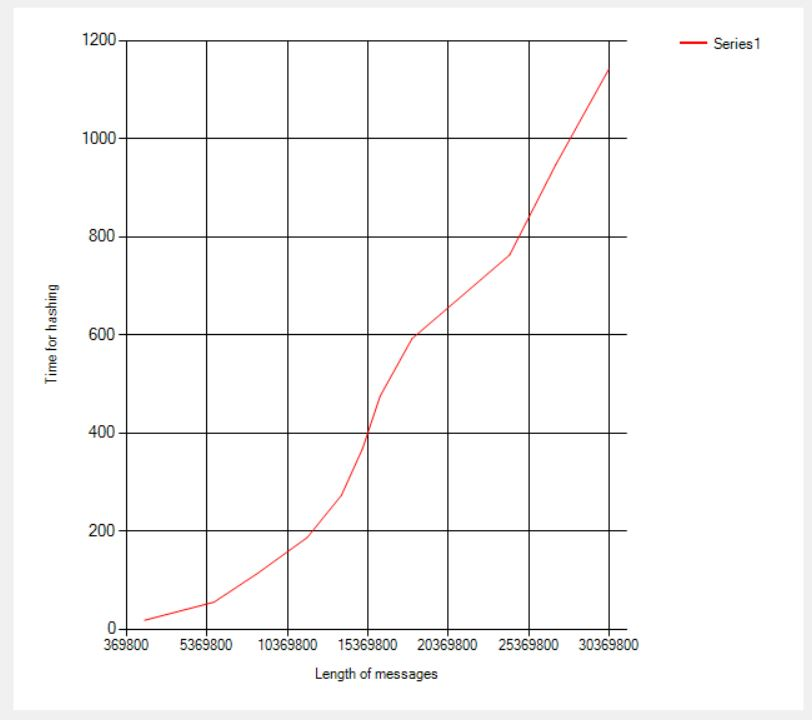
\includegraphics[scale=0.4]{S4Q1}
            \caption{plot of time vs length of content}
            \label{fig:SHA256 timing vs content length}
        \end{figure}
        
    \paragraph{Question 2:} Compute the Merkle tree (directly) over files $F = (F_1; F_2; . . . ; F_8)$ where $F_i$ is the i-th posted .pdf file with lecture slides for CS579. What is the digest \emph{d}, i.e., the hash of the tree root? What is the average proof size and what is the average verification time, measured over all possible queries $i = 1; 2; . . . 8$? How does such average performance compare against the asymptotic proof size and verification time that Merkle trees provide?    
    \paragraph{Answer:\newline}
        The digest \emph{d} of Merkle tree when calculated over files directly is as \newline 6D80A9318F50BFFC4990A94DA216A8F6677C9D3A8AD22912B7EFB94C00232513.
        
    \paragraph{Question 3:} Compute the Merkle tree (directly) over the hashed files $h = (h_1; h_2; . . . ; h_8)$ where $h_i = h(F_i)$, i = 1; 2; . . . 8, and $F_i$ are as before. What is the digest $d^\prime$, i.e., the hash of the tree root? What is the average proof size and what is the average verification time, measured over all possible queries i = 1; 2; . . . 8? How does these averages compare with the worst-case corresponding values?
    \paragraph{Answer:\newline}
        The digest \emph{d} of Merkle tree when calculated over hash of files is as \newline 1C47F4F9E19156534EE48DCC0DDCD3EA400170E5EE53C19299B60F3EC8141E8C. 
    
    
    \paragraph{Question 4:} Assume that the user wants to be able to have \emph{secure} access to its outsourced files F also from a different device $D^\prime$, but simply migrating the digest \emph{d} to device $D^\prime$ from the existing device \emph{D} is not possible. How the use of public-key cryptography can provide a solution to this problem?
    \paragraph{Answer:\newline}
    
\bibliographystyle{plain}
\bibliography{references}

\end{document}
